
\documentclass[12pt]{article}
\usepackage[margin=1in]{geometry}
\usepackage[english]{babel}
\usepackage[utf8x]{inputenc}
\usepackage{amsmath}
\usepackage{amsfonts}
\usepackage{amssymb}
\usepackage{parskip}
\usepackage{rotating}
\usepackage{natbib}
\usepackage{subfigure}
\usepackage{tikz}
\usepackage{graphicx}
%% PATH TO FIGURES and TABLES
\graphicspath{ {./Exhibits/} }

\usepackage{watermark}
\thiswatermark{\centering \put(-70,-749){
\includegraphics[scale=1]{cover.png}} }
\usepackage{titlesec}
\usepackage{xcolor}
\titleformat*{\section}{\filcenter\Large\bfseries\sffamily\color{red}}
\titleformat*{\subsection}{\large\bfseries\sffamily\color{red}}
\titleformat*{\subsubsection}{\sffamily\color{red}}
\usepackage{fancyhdr}
\pagestyle{fancy}
\usepackage{pdfpages}
%\usepackage{apacite}
% 508 Compliance
%\usepackage{pdfcomment}
\usepackage{accsupp}

%% ENTER SHORT TITLE for RUNNING HEAD
\lhead{\textsf{ }} % controls the left corner of the header
%%
\cfoot{} % controls the center of the footer
\rhead{\textsf{Page~\thepage}} % controls the right corner of the footer
 

\begin{document}


\thispagestyle{empty}
\cleardoublepage{}

\hspace{-2cm}\begin{minipage}[b]{0.3\linewidth}
\begin{flushleft}
 
\vspace{6cm}

%%% ENTER AUTHOR NAMES HERE   
\textsf{ } \\
\textsf{ } \\
\end{flushleft}
\end{minipage}

\hspace{5cm}\begin{minipage}[t]{0.8\textwidth}
\begin{center}

%%% ENTER TITLE HERE
\Large{\textbf{\textsf{WI22-QTP: Economic Security of People with Disabilities during the Pandemic }}}\\
\end{center}
\end{minipage}

\hspace{5cm}\begin{minipage}[t]{0.7\textwidth}


\begin{flushleft}
\vspace{6cm}

%% STANDARD DISCLAIMER
\footnotesize{\textsf{The research reported herein was performed pursuant to a grant from the U.S. Social Security Administration (SSA) funded as part of the Retirement and Disability Consortium. The opinions and conclusions expressed are solely those of the author(s) and do not represent the opinions or policy of SSA or any agency of the Federal Government. Neither the United States Government nor any agency thereof, nor any of their employees, makes any warranty, express or implied, or assumes any legal liability or responsibility for the accuracy, completeness, or usefulness of the contents of this report. Reference herein to any specific commercial product, process or service by trade name, trademark, manufacturer, or otherwise does not necessarily constitute or imply endorsement, recommendation or favoring by the United States Government or any agency thereof.}}
\end{flushleft}

\end{minipage}
 


\cleardoublepage{}

% SPACING 
\linespread{1.25} 
\section*{Abstract}
		\noindent   
		
				\noindent\textbf{JEL Classification Codes:} I31, I32, R21. \\
		\noindent\textbf{Keywords:}    Social Security\\

\newpage 
 
\section{Introduction}


\includegraphics[scale=0.65]{}


\subsection{Background}

 
 
 
There are multiple paths through which the COVID-19 pandemic may affect the economic security of working age adults with disabilities. Disruptions to the economy and risk of disease spread led some who were working prior to the pandemic to exit the labor market \citep{cheng2020back, goda2021impact moen2020disparate, quinby2021older }, thereby reducing income through wage earnings. This reduction in labor force participation has not been offset by a subsequent increase in Social Security  claiming [CITE?].   


Reduced consumption \citep{baker2020does,horvath2021covid} 

households often unable to pay their bills \citep{clark2021financial,schneider2020household}. 

  
We begin our analysis by  

We further explore mechanisms underlying changes 

 

Taken together, the results of this study provide important detail about the depth and breadth of the inequity of financial hardship experienced in the pandemic. Our findings indicate heterogeneous effects for vulnerable segments of the population.    


\cite{adams2020inequality,andersen2020consumer,andersen2020pandemic,baker2020does,bhutta2020covid,braxton2020can,brewer2020initial,casado2020aggregate,cheng2020back,cherry2021government,chetty2020did,clark2021financial,coibion2020labor,cfpb2020,cowan2020short,cutts2020musings,emerson2021impact,enriquez2020covid,farrell2020consumption,findling2021serious,gerardi2021racial,gignac2021impacts,goda2022impact,goda2021impact,grantz2020use,haughwout2020us,horvath2021covid,li2020impact,loibl2020role,lusardi20186,moen2020disparate,mullen2022economic,quinby2021older,schneider2020household,schur2021covid,stavins2021unprepared}

\section{ Prior Literature}

 

\subsection{COVID-19 and  Financial Security  }

There is a burgeoning body of literature on the economic consequences of the COVID-19 pandemic for U.S. households. Most directly, several studies analyze changes in labor force participation and unemployment in response to the COVID-19 pandemic (e.g.  \cite{cheng2020back}), with a few studies focusing on labor trends  \citep{goda2021impact,moen2020disparate,quinby2021older}.   

Reductions in income may be offset in part by reductions in consumption  \citep{baker2020does,casado2020aggregate,chetty2020did,farrell2020consumption,horvath2021covid}. For example, \cite{farrell2020consumption} find an overall 10 percent decline in consumer spending following the onset of the pandemic. However, the effects on consumption are heterogeneous across a number of dimensions.  \cite{chetty2020did} find that much of the reduction in spending is concentrated among higher income households—households in the top income quartile spent 13 percent less as of mid-July 2020 relative to January 2020, whereas households in the bottom income quartile reduced consumption by only 4 percent during the same period. For those experiencing a COVID related loss of income, \cite{farrell2020consumption} find that receipt of pandemic-related unemployment benefits is associated with a 10 percent increase in consumer spending relative to the prior year. 


 
 
 Emerson and colleagues studied the effects of pandemic  on people with disabilities in the UK ‘Understanding Society’, an annual household panel study \citep{emerson2021impact}. Respondents with disability were more likely to experience higher levels of financial stress.  

 Gignac and colleagues studied people with physical or mental health disabilities in Canada. People with a  disability reported more  financial concerns, more contract work, and unmet accommodations at work  than those with no disability. \citep{gignac2021impacts}

  Goda, et al sue Current Population Survey and monthly Google Trends data to show fewer labor force exits due to disability and applications for disability insurance \citep{goda2022impact}


\citeauthor{schur2021covid} find White and Black women with disabilities experienced relatively greater employment losses during the pandemic compared to White men without disabilities. \citep{schur2021covid}

   \cite{cowan2020short} also finds workers with a disability—have experienced the largest declines in the likelihood of (full-time) work and work hours.

  
Kathleen Mullen and Nicole Maestas
 
Previous economic downturns have led to increases in applications for and, eventually, receipt of Social Security Disability Insurance (SSDI) benefits. In the pandemic-induced recession of 2020 and its aftermath, however, SSDI applications did not increase. One important factor may have been the prolonged closure of SSA field offices, since previous research finds that field office closures lead to persistent declines in SSDI beneficiaries in the surrounding communities. In this case, there may be pent-up demand for SSDI benefits as normal operations resume in areas where the economy has not fully recovered. Government support programs were materially different than in past recessions, which appears to have enabled people to weather the downturn and avoid applying for SSDI benefits. \cite{mullen2022economic}

 


 
 
\section{Data and Methods}
We explore the differences in financial wellbeing of households with and without disabilities in two different time periods. First, we use two datasets that are repeated cross sections, allowing us to compare households with and without disabilities before and after the start of the pandemic. Second, we use individual-level data that is recorded monthly starting in the spring of 2020. This tells us more about the evolution of the gap between households with and without disabilities throughout the pandemic. 

\textcolor{blue}{DO WE SAY SOMETHING ABOUT THE THREE DIFFERENT MEASURES OF DISABILITY?}


We explain each data and empirical strategy next. 

\subsection{Before and After Pandemic Changes}
We use two datasets to explore the differences in financial security for those with and without disabilities before and after the pandemic. 

First, we use the National Financial Capability Study (NFCS) data, a nationally-representative survey conducted every three years by the FINRA Investor Education Foundation. We use data from the 2018 and 2021 waves, as they include information on disability status, as well as financial wellbeing. The 2021 survey was conducted in the late summer to early fall. We consider a respondent to have a disability if they answered ``Permanently sick, disabled, or unable to work" to the question ``Which of the following best describes your current employment or work status?" We recognize that this is a relatively broad definition of disability. In order to examine a sample that is working-age, we limit our respondents to those between 18 and 64 years of age. 

We define five main variables of interest in this sample that all reflect the financial security of the household: presence of emergency savings, financial anxiety, whether they made a late credit card payment, whether they used alternative financial services, and the U.S. Consumer Financial Protection Bureau's financial wellbeing scale (FWB). The first four are dummy variables. FWB is measured from 0 to 100, based on the answers to five questions related to one's ability to keep up with day-to-day or month-to-month finances, as well as individual expectations of their ability to meet future financial goals.\footnote{For more on the FWB measure, see \url{https://www.consumerfinance.gov/consumer-tools/financial-well-being/about/}.}  Summary statistics for the NFCS data are in Appendix Table \ref{NFCS_Summstats}. 


To investigate how the FWB score changed before and after the pandemic for the respondents with disabilities as compared to the same for the respondents without disabilities, we estimate the following model:

\begin{equation}\label{eqn1}
Y_{it}=\alpha+\beta_0 Disability_i + \beta_1 Post_t+ \beta_2 Disability_i \times Post_t +\gamma X_i + \epsilon_{it} 
\end{equation}

where $Y_{it}$ refers to the outcome variable for respondent $i$ in year $t$, $Disability_i$ is an indicator which takes a value of 1 for the respondents with disabilities and a 0 otherwise, and $Post_t$ is an indicator which takes a value of 1 for the post-pandemic year (2021) and a 0 otherwise. The coefficient of interest is $\beta_2$ which shows the difference in post-pre change in financial well-being outcomes between respondents with and without disabilities after the pandemic started. Equation \ref{eqn1} includes individual-level control variables, including dummies for race/ethnicity, gender, and income buckets. 

Second, we use data from the Survey of Household Economics and Decisionmaking (SHED) 2018-2021 provided by the Federal Reserve Board. We identify respondents with disabilities if they answered \emph{yes} to the question ``Did health/medical limitations or disability contribute to you not working / not working as much as you wanted last month?'' Again, we limit our sample to respondents aged between 18 and 64. We consider four SHED questions related to financial hardship. Table \ref{table:SHED.ques.table} provides a description of the these questions with the response options. Combining respondents who answered all the key questions in SHED 2018-2021, we get a sample of 10,983 respondents. Appendix Table \ref{SHED_Sumstats} provides summary statistics for the SHED analytical sample. We continue to estimate a version of Equation \ref{eqn1}, in which $Post$ refers to observations from SHED 2020 (conducted in November 2020) and 2021 (conducted between October and November 2021). 

% Please add the following required packages to your document preamble:

%    \resizebox{6in}{!}{%

\begin{table}[!ht]
    \centering
    \caption{Description of Survey of Household Economic Decisionmaking (SHED) questions}
    \resizebox{6in}{!}{%
    \begin{tabular}{lll}
    \hline
        Question & Response Options & Binary Coding \\ \hline
        In the past month, would you say that your & More than your income & 1 \\ 
        total spending was: & The same as your income & 0 \\ 
        ~ & Less than your income & 0 \\ 
        ~ & ~ & ~ \\ 
        Compared to 12 months ago, would you & Much worse off & 1 \\ 
        say that you (and your family) are better & Somewhat worse off & 1 \\ 
        off, the same, or worse off  & About the same & 1 \\ 
        financially? & Somewhat better off & 0 \\ 
        ~ & Much better off & 0 \\ 
        ~ & ~ & ~ \\ 
        Overall, which one of the following best & Finding it difficult to get by & 1 \\ 
        describes how well you are managing  & Just getting by & 1 \\
        financially these days? & Doing okay & 0 \\
        ~ & Living comfortably & 0 \\ 
        ~ & ~ & ~ \\ 
        In the past 12 months, how frequently  & Most or all of the time & 1 \\ 
        have you carried an unpaid balance on  & Some of the time & 1 \\ 
        one or more of your credit cards? & Once & 1 \\ 
        ~ & Never carried an unpaid balance & 0 \\ \hline
    \end{tabular}}
    \label{SHED.ques.table}   
\end{table}


\subsection{Within Pandemic Changes}

This paper uses data from the Household Pulse Survey (HPS) to investigate whether financial hardship worsened among people with disabilities compared to people without disabilities over the pandemic. The U.S. Census Bureau collaborated with multiple other federal agencies to conduct the HPS. The key objective of the survey was to quickly and efficiently gather data on the hardships faced by American households during the pandemic. Although the HPS provides a rich source of data collected over regular intervals from April 2020 to the time of writing this paper, it does not have a variable that directly identifies people with disabilities. We use the Medicare eligibility rule for non-elderly adults to identify the respondents with disabilities. Specifically, we identify a respondent as a person with disability if they meet two conditions: 1) aged between 19 and 64 and 2) enrolled in Medicare. Although this approach helps us correctly identify a segment of the respondents with disabilities, it cannot detect all the respondents with disabilities. 

In terms of outcomes of interest, we use three variables related to financial hardship: 1) food insufficiency in the last seven days, 2) difficulty with financial expenses in the last 7 days, and 3) confidence in paying the next month's rent/mortgage payments. The question on food insufficiency asks:  `` In the last 7 days, which of these statements best describes the food eaten in your household? Select only one answer.'' The response options are 1) enough of the kinds of food (I/we) wanted to eat, 2) enough, but not always the kinds of food (I/we) wanted to eat, 3) sometimes not enough to eat, and 4) often not enough to eat. We create a \emph{food insufficiency} indicator variable, which takes a value of 1 if the respondent selected either sometimes not enough to eat or often not enough to eat and a otherwise. The question on difficulty with financial expenses asks: ``In the last 7 days, how difficult has it been for your household to pay for usual household expenses, including but not limited to food, rent or mortgage, car payments, medical expenses, student loans, and so on? Select only one answer.'' The response options are: 1) not at all difficult, 2) a little difficult, 3) somewhat difficult, and 4) very difficult. We create a \emph{difficulty with expenses} indicator variable, which takes a value of 1 if a respondent selected either somewhat difficult or very difficult and 0 otherwise. Finally, the question on confidence in paying next mortgage/rent payment asks: ``How confident are you that your household will be able to pay your next rent or mortgage payment on time? Select only one answer.'' The response options are 1) not at all confident, 2) slightly confident, 3) moderately confident, and 4) highly confident. We create a \emph{not confident in paying mortgage/rent} indicator variable, which takes a value of 1 if the respondent selected either not at all confident or slightly confident and 0 otherwise.

\subsubsection{Analytical Samples}
As the sample sizes at the individual HPS week level get smaller, we combine respondents from multiple HPS weeks to create quarterly (trimonthly) samples. Table \ref{table:period.table} provides a description of the coding of these quarterly periods. We create three analytical samples based on the responses to the three questions of interest. Appendix tables \ref{hps_food_sample}-\ref{hps_mortgage_sample} provide the summary statistics for the HPS data.   

\begin{table}[ht]
\centering
\caption{Coding of Quarterly Periods}\label{table:period.table}
\begin{tabular}{lll}
\hline
\textbf{Quarterly Periods} & \textbf{HPS Weeks} & \textbf{Months, Year} \\
\hline
1                          & 1-9                  & April-June, 2020               \\
2                          & 10-15                & July-September, 2020           \\
3                          & 16-21                & October-December, 2020         \\
4                          & 22-27                & January-March, 2021            \\
5                          & 28-33                & April-June, 2021               \\
6                          & 34-38                & July-September, 2021           \\
7                          & 39-40                & October-December, 2021\\
\hline
\end{tabular}
\end{table}

For the food insufficiency sample, we combine respondents from HPS weeks 1 to 40, which has a total sample of 3,192,531 respondents. Next, we narrow it down to respondents aged between 19 and 64 who responded either yes or no to the Medicare coverage question, which results in a sample  of 1,732,037 respondents. Finally, we eliminate those who did not answer the food insufficiency question and get a sample of 1,729,108 respondents. \\
\\
As the HPS started asking the difficulty with expenses question from week 13 onward, for the difficulty with expenses sample, we combine respondents from HPS weeks 13 to 40, which have a total sample of 2,104,217 respondents. After narrowing it down to respondents aged between 19 and 64 who responded either yes or no to the Medicare coverage question, we get a sample of 1,106,186 respondents. Among these respondents, a total of 1,104,824 answered the difficulty with expenses question. \\
\\
For the confidence in paying next rent/mortgage payments sample, we combine respondents from HPS weeks 1 to 40 for whom the tenure status was either \emph{owned with a mortgage or loan (including home equity loans)} or \emph{rented} (sample size=1,962,199). Narrowing it down to respondents aged between 19 and 64 who responded either yes or no to the Medicare coverage question results in a sample of 1,400,608 respondents. The analytical sample for analyzing the confidence in paying rent/mortgage outcome consists of 1,395,349 respondents who answered the confidence in paying rent/mortgage question.

\subsubsection{Estimation}
To investigate whether the financial hardships faced by people with disabilities worsened over time compared to people without disabilities, we estimate the following model: \\
\begin{equation}\label{eqn2}
Y_{it}= \alpha_0+\alpha_1 Disability_i+\sum_{t=2}^{7} \beta_t Period_t+\sum_{t=2}^{7} \gamma_t Disability_i \times Period_t
+e_{it} 
\end{equation}

where $Y_{it}$ refers to the value of the outcome variable for respondent $i$ in period $t$, $disability_i$ is a dummy variable which takes a value of 1 if respondent $i$ is both aged 19-64 and enrolled in Medicare, and a 0 otherwise, $period_t$ refers to a vector of dummy variables which take a value of 1 for the quarterly period $t$ and a 0 otherwise. We are primarily interested in the coefficients of the interaction terms ($Disability_i \times Period_t$), comparing the difference across people with and without disabilities in each given period compared to period one.  \\


This approach helps us explore the extent to which the gap in the three outcome variables between the two groups evolved over time in the first two years of the pandemic. We estimate equation \ref{eqn2} with and without  control variables. The control variables are state of residence, gender, pre-tax annual household income in buckets, race, Hispanic status, age, homeownership status, marital status, educational attainment, number of dependents below 18, and household size.



\section{Findings}
\subsection{Before and After Pandemic Changes}
We use two different surveys that capture different measures of economic and financial security, different measures of disability, and different points in time post-pandemic. In the NFCS, disability represents those who were ``permanently sick, disabled, or unable to work." In the SHED, disability represents those who had health or medical limitations that prevented them from working that month. Thus, the NFCS captures a population with  more long-term problems, and the SHED has a more inclusive measure that contains those with short-term medical limitations. The SHED 2020 and 2021 surveys took place in the fall of each year, and the NFCS surveys took place late summer of 2021. 

\subsubsection{NFCS Findings}

Beginning with the NFCS, Figure \ref{NFCS_Y} shows the difference in financial outcomes across 2018 and 2021 for respondents with and without disabilities. The changes are measured in percentage point differences, since each outcome is a dummy variable. While both groups were more likely to have emergency savings in 2021 than 2018, those without disabilities experienced a greater increase.\footnote{The full question is: Have you set aside emergency or rainy day funds that would cover your expenses for 3 months, in case of sickness, job loss, economic downturn, or other emergencies?} At the same time, financial anxiety increased by more for people without disabilities than people with disabilities. A similar story exists for AFS use, which includes payday loans, pawn shops, tax return advances, and rent-to-own services. However, the AFS measure asks about the last five years, making it potentially less of a pandemic story and a more overall trend. Both groups saw an equal increase in the likelihood of having a credit card with a late payment, conditional on having a credit card. Taken together, these findings suggest that though households are more likely to have three months of savings in case of emergencies, they are more  anxious about the future of their financial situation than they were three years prior. While households with disabilities were more likely to be financially anxious than before the pandemic started, the change in their experiences are less severe than people without disabilities. This could be because SSA's programs provide a guarantee of future income for households with disabilities. 

We next look at subjective measures in Figure \ref{NFCS_FWB} in the CFPB's FWB score. Overall, people with disabilities saw an improvement in FWB, while people without disabilities saw a small decrease in FWB. The only measure within the scale that respondents with disabilities did worse on in 2021 than 2018 was thinking the money they had or will save won't last. This matches the financial anxiety increase, suggesting that there is concern for the future. However, people with disabilities were less likely to say they were just getting by financially, they will never have the things they want in life because of money, and their finances controlled their lives. They were more likely to say they had money left over at the end of the month, consistent with the finding from Figure \ref{NFCS_Y} that respondents with disabilities had more emergency savings in 2021 than 2018. 

Overall, these findings suggest that while the ability to keep up with month-to-month and day-to-day finances improved for respondents with disabilities from 2018 to 2021---particularly when compared to those without disabilities---they remain more anxious about their financial future than in the past. The 2021 survey took place over a year into the pandemic, but worldwide changes due to the pandemic could have made people more uncertain about the future. On every marker except for emergency savings, respondents with disabilities had less detrimental changes from 2018 to 2021. 

\subsubsection{SHED Findings}
%%Fix the figure (SHED barplots) label%% 
Figure \ref{shed.desc.graph} shows the post- and pre-pandemic changes in financial hardships for respondents with and without disabilities. All the outcomes are coded as binary variables for which 1 refers to a higher level of financial hardship. We observe that the respondents with disabilities are less likely to spend more than income in the post-pandemic period, whereas there is no change in the same outcome for the respondents with no disabilities. Although both groups are less likely to mention greater hardship while responding to the question on how they are managing their finances (\emph{difficult to get by}), the decrease is higher for the respondents with disabilities. Surprisingly, both groups mention higher hardship while answering the question on whether they are better off/the same/worse off financially compared to 12 months ago (\emph{no better off}); however, the increased likelihood of greater hardship is lower for respondents with disabilities. Finally, we observe no changes in the incidence of carrying an unpaid balance on one or more of credit cards (conditional on having at least one credit card) in the past 12 months for the respondents with disabilities. Interestingly, we observe a drop in the same outcome for the respondents with no disabilities. Overall, these findings imply that there were less detrimental pre- and post-pandemic changes in financial hardships for people with disabilities except for the no change in the incidence of carrying some credit card balance. 

Table \ref{table:shed.reg.table} shows the results obtained by estimating equation (\ref{eqn1}) on the four outcome variables from the SHED. We observe statistically significant decreases in \emph{difficult to get by} and \emph{no better off} outcomes and a significant increase in \emph{credit card balance} outcome for the respondents with disabilities; however, we do not observe any significant change in the (\emph{Spend$>$Income}) outcome for the respondents with disabilities. In general, the regression findings align with the descriptive findings. 

\subsection{Within Pandemic Changes}

Figures \ref{food_insuf_desc}-\ref{mort_conf_desc} show the trends in the three outcome variables for the respondents with and without disabilities. Descriptively, it appears that for the food insufficiency and difficulty with expenses variables, the gap in the average value between the two groups remained almost the same. For the confidence in paying next rent/mortgage payment variable, the gap in the average value between the two variables remained the same except in the last two quarterly periods, in which respondents with disabilities apparently reported lower confidence. Figures \ref{food_insuf_wc}-\ref{rent_conf_wc} show the extent to which the gap in the three outcome variables between people with and without disabilities changed over the quarterly periods relative to period 1 (April-June 2020). In figure \ref{food_insuf_wc}, we observe that the estimated coefficient is not significantly different from 0 at the 5 percent significance level in any of the periods except in period 6 (July-September 2021), which suggests that the gap in food insufficiency for the two groups remained mostly the same throughout the pandemic. Figure \ref{expens_dif_wc} shows similar trends for the difficulty with expenses variable. Lastly,  figure \ref{rent_conf_wc} shows that for the rent/mortgage confidence variable, there was no significant change in the gap in the outcome between the two groups until period 5 relative to period 1; however, we do observe increasing gap in the outcome between the two groups in the last two periods (between July and December 2021) relative to period 1. Overall, these findings indicate that the financial hardship faced by the people with disabilities was not disproportionately higher for the most parts over the studied period. 

\section{Conclusion}
 
Implications for Social Security Programs
 
Increased eligibility for SSI and Medicaid, as well as SNAP and LIHEAP

PWD are more anxious  - but maybe not living as long - foregone health care - future outcomes could be negative - changing trajectories

Look for papers on health, DI, SSI - what are trends in anxiety and other measures of distress

SSA benefits are more secure and should  be more stable for most people  - anxiety could be related to other HH members

HHs with someone who has disability are not able to take advantage of strong labor markets relative to non disabled

Look at tables of BRFSS

\cite{blanchflower2022covid}

SSA will find higher levels of distress among SSDI and SSI recipients 

Implications - National Disability Institute programs for financial capability


\cite{kruse2022disability}
Remote work may help people with disabilities with labor force
People with disabilities experienced relatively more pandemic-related hardships compared to people without disabilities

more difficulty in accessing medical care.

comorbidities, including poor mental health,

access to home and community-based services 

 care coordination  with financial supports
 
 \cite{mitra2022advancing}
 

\section{Figures and Tables}
 
 \begin{figure}[h!]\label{SHED_Y}
\caption{Changes in Financial Outcomes Pre- and Post- Pandemic across People with and without Disabilities (SHED)}
\centering
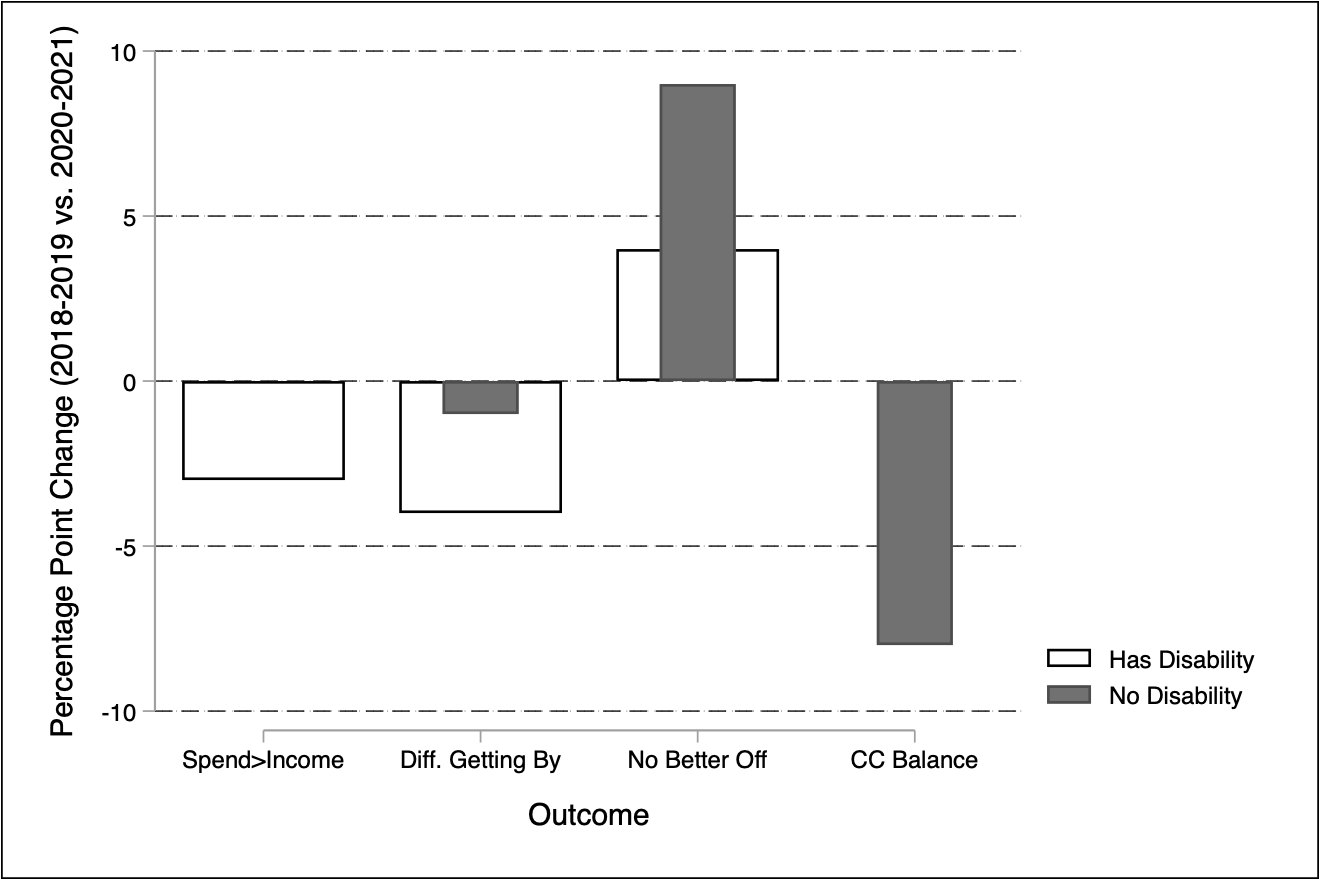
\includegraphics[scale=0.4]{Exhibits/SHEDChange_DisNoDis.png}
\medskip 
\begin{minipage}{0.65\textwidth} 
{\footnotesize Notes: Data come from the 2018--2021 SHED. Each bar represents the difference in the average measure for people with and without disabilities pre- (2018--2019) and post- (2020--2021) pandemic in percentage point terms. Spend$>$ Income equals one if the individual reported spending more than income in the past month and zero otherwise. Diff. Getting By equals one if the individual is finding it difficult to get by or just getting by and zero otherwise. No Better Off equals one if the individual reports being no better off financially than 12 months prior and zero otherwise. Credit card balance equals one if the individual has a credit card balance and zero otherwise. \par}
\end{minipage}
\end{figure}

\begin{figure}[h!]\label{NFCS_Y}
\caption{Changes in Financial Outcomes from 2018-2021 across People with and without Disabilities (NFCS)}
\centering
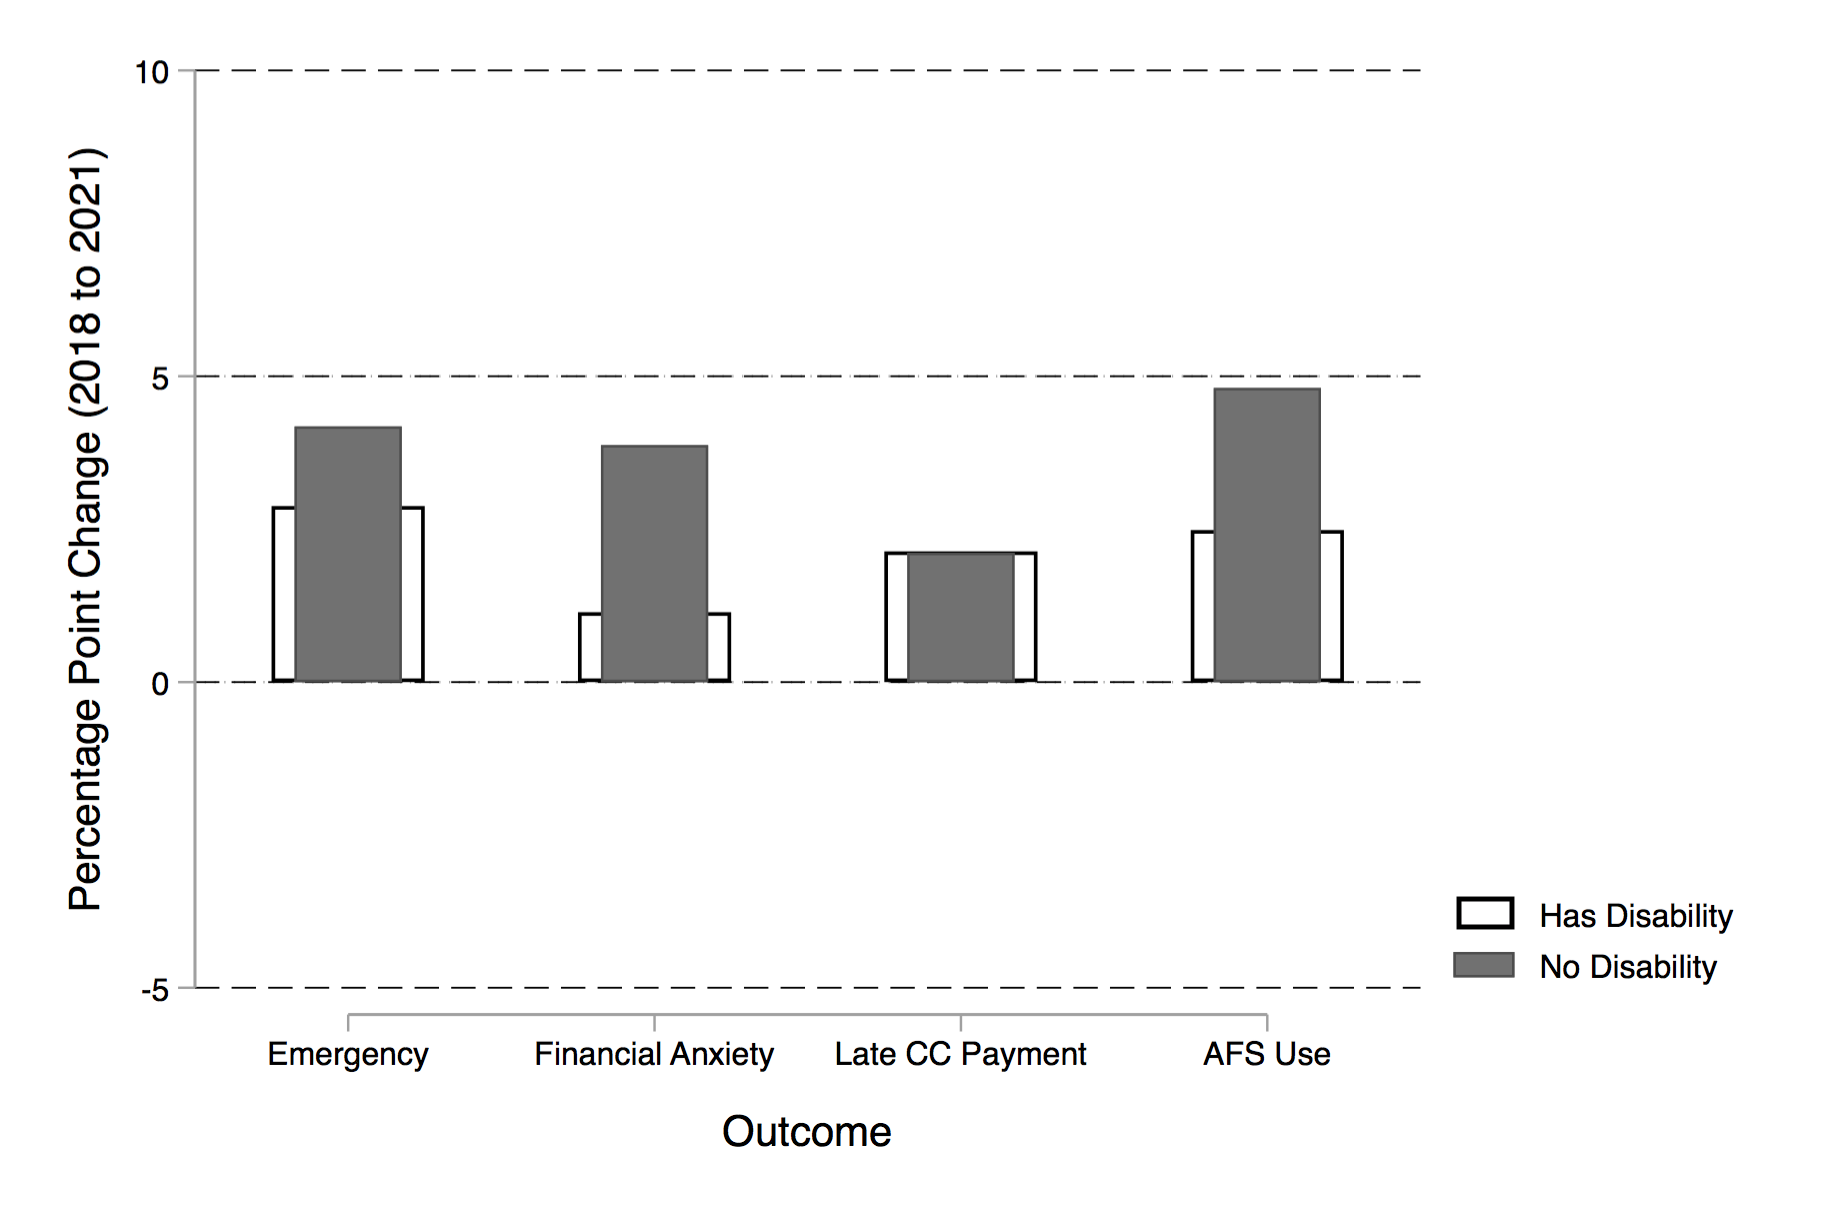
\includegraphics[scale=0.4]{Exhibits/ChangeY_18_21_NFCSdisabilitynodis.png}
\medskip 
\begin{minipage}{0.65\textwidth} 
{\footnotesize Notes: Data come from the 2018 and 2021 NFCS. Each bar represents the difference in the average measure for people with and without disabilities from 2018 to 2021 in percentage point terms. Emergency is whether someone has emergency savings. Financial anxiety is whether the individual agreed with the following statement: ``discussing my finances can make my heart race or make me feel stressed." Late CC Payment is whether someone was charged a late fee on their credit card. AFS use is whether the individual used a payday lender, pawn shop, tax return advance, or rent-to-own service in the past five years.   \par}
\end{minipage}
\end{figure}

\begin{figure}[h!]\label{NFCS_FWB}
\caption{Changes in Financial Wellbeing from 2018-2021 across People with and without Disabilities (NFCS) }
\centering
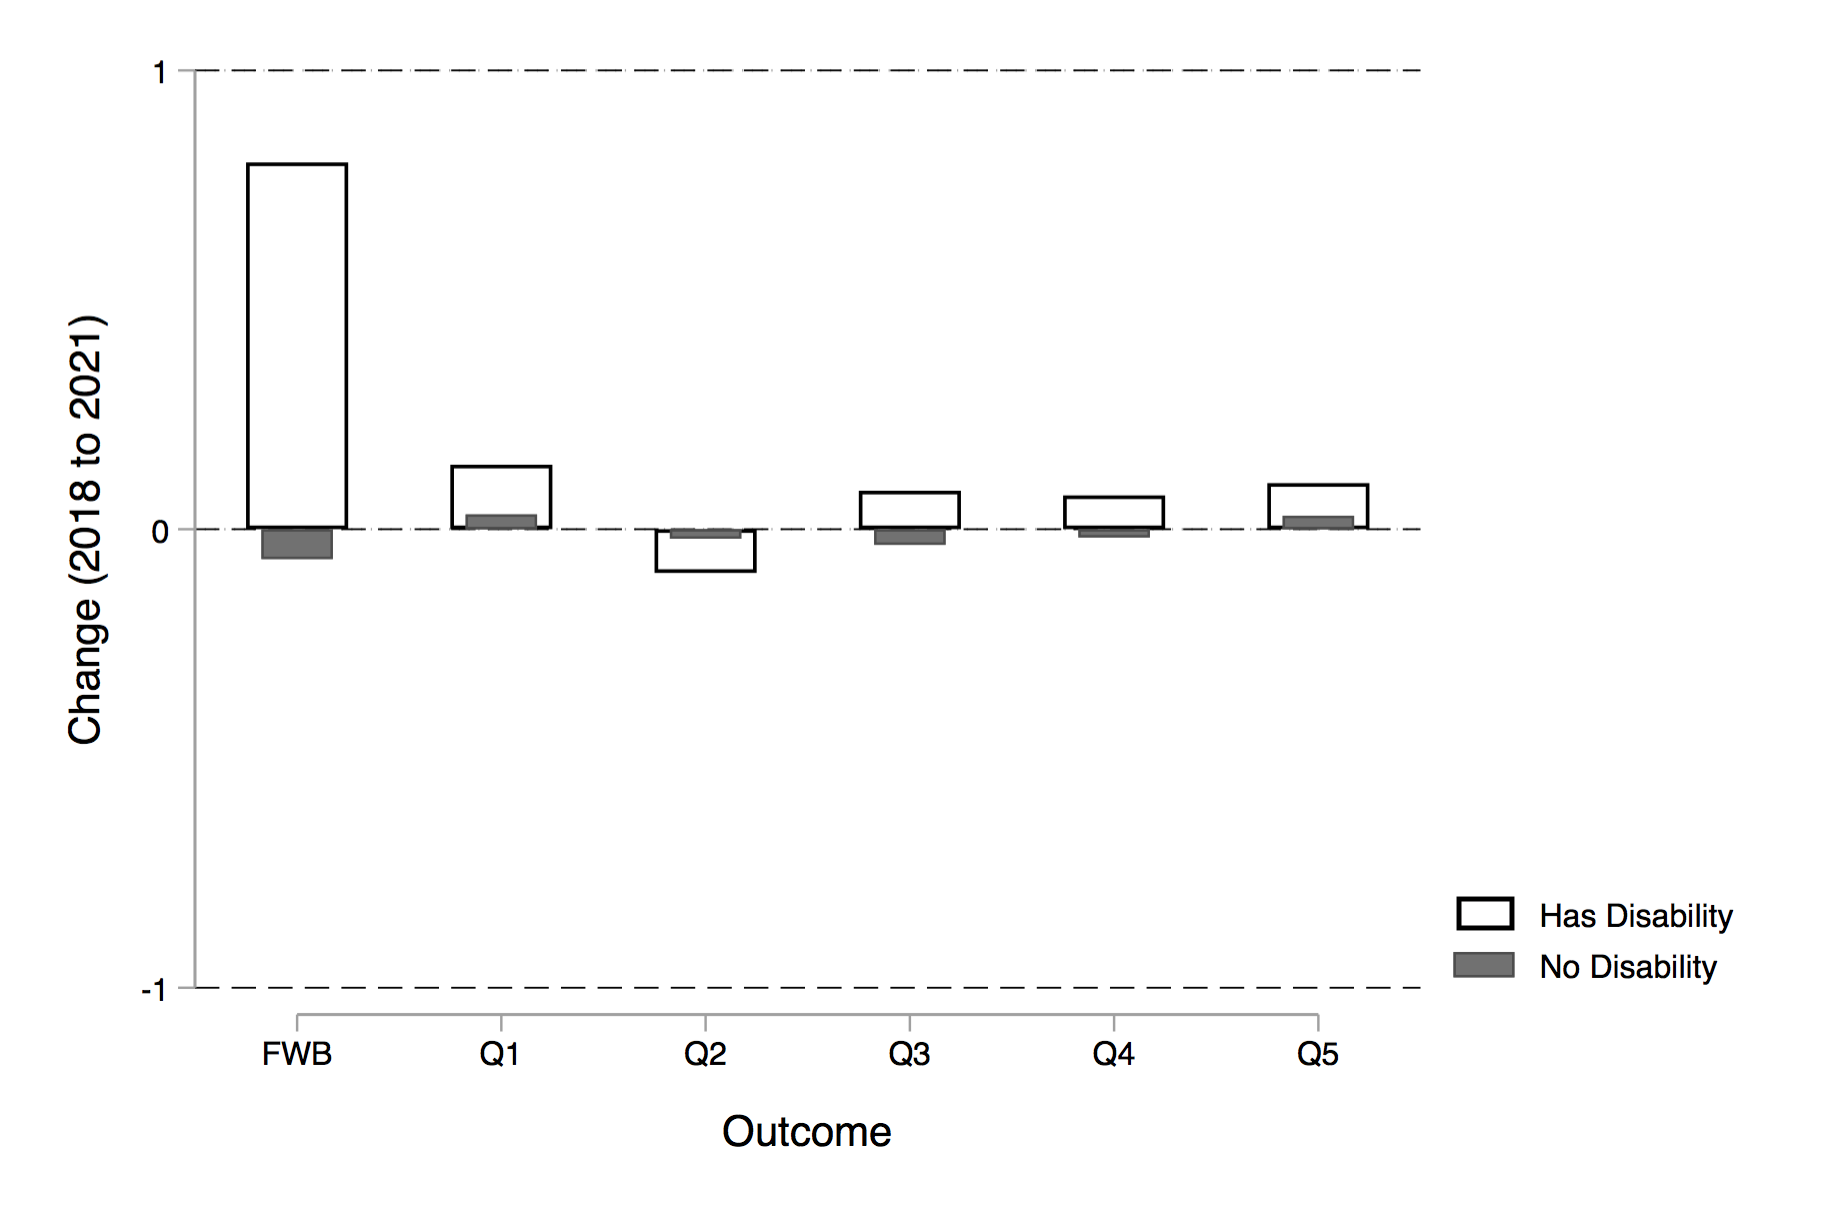
\includegraphics[scale=0.4]{Exhibits/ChangeFWB_18_21_NFCSdisabilitynodis.png}
\medskip 
\begin{minipage}{0.65\textwidth} 
{\footnotesize Notes: Data come from the 2018 and 2021 NFCS. Each bar represents the difference in the average measure for people with and without disabilities from 2018 to 2021. Financial Well-being measured from 0 to 100. Each component of Financial Well-being are the following five questions. These are scaled from 0 to 4, where higher scores are recoded to always be better. Q1: I am just getting by financially; Q2: I am concerned the money I have or will save won't last; Q3: Because of my money situation, I feel like I will never have the things I want in life; Q4: My finances control my life; Q5: I have money left over at the end of the month. \par}
\end{minipage}
\end{figure}
\clearpage

\begin{table}\label{NFCS_regs}
\caption{Changes in Outcomes Post-Pandemic Across Households with and without Disabilities}
{
\def\sym#1{\ifmmode^{#1}\else\(^{#1}\)\fi}
\begin{tabular}{l*{5}{c}}
\hline\hline
                    &\multicolumn{1}{c}{(1)}&\multicolumn{1}{c}{(2)}&\multicolumn{1}{c}{(3)}&\multicolumn{1}{c}{(4)}&\multicolumn{1}{c}{(5)}\\
                    &\multicolumn{1}{c}{Financial }&\multicolumn{1}{c}{Emergency }&\multicolumn{1}{c}{Fin. }&\multicolumn{1}{c}{Late CC }&\multicolumn{1}{c}{Used }\\ &\multicolumn{1}{c}{ Well-being}&\multicolumn{1}{c}{ Savings}&\multicolumn{1}{c}{ Anxiety}&\multicolumn{1}{c}{ Payment}&\multicolumn{1}{c}{AFS}\\
\hline
Post                &       0.348\sym{**} &       0.053\sym{***}&       0.036\sym{***}&       0.016\sym{***}&       0.044\sym{***}\\
                    &     (0.172)         &     (0.005)         &     (0.006)         &     (0.004)         &     (0.006)         \\
[1em]
Has Disability      &      -7.219\sym{***}&      -0.153\sym{***}&       0.101\sym{***}&       0.023         &       0.114\sym{***}\\
                    &     (0.324)         &     (0.010)         &     (0.012)         &     (0.017)         &     (0.013)         \\
[1em]
Has Disability x Post&       0.701         &      -0.015         &      -0.026         &       0.005         &      -0.024         \\
                    &     (0.534)         &     (0.014)         &     (0.017)         &     (0.024)         &     (0.017)         \\
\hline
Observations        &       42779         &       43196         &       43196         &       33054         &       43196         \\
\hline\hline
\end{tabular}
}
\medskip 
\begin{minipage}{0.85\textwidth} 
{\footnotesize Notes: Coefficients reported with standard deviations in parentheses. Data come from the 2018 and 2021 NFCS. FWB measured from 0 to 100. Each bar represents the difference in the average measure for people with and without disabilities from 2018 to 2021 in percentage point terms. Emergency is whether someone has emergency savings. Financial anxiety is whether the individual agreed with the following statement: ``discussing my finances can make my heart race or make me feel stressed." Late CC Payment is whether someone was charged a late fee on their credit card. AFS use is whether the individual used a payday lender, pawn shop, tax return advance, or rent-to-own service in the past five years. Post represents 2021, where the exlcuded group is 2018. We consider a respondent to have a disability if they answered ``Permanently sick, disabled, or unable to work" to the question ``Which of the following best describes your current employment or work status?" \sym{*} \(p<0.10\), \sym{**} \(p<0.05\), \sym{***} \(p<0.01\) \par}
\end{minipage}
\end{table}

%%%%%%%%%%% SHED Regression table %%%%%%%%%%%
%\resizebox{6in}{!}{%

\begin{table}[]
\centering
\caption{Pre and post pandemic change in financial well-being between people with and without disabilities}\label{table:shed.reg.table}
{
\def\sym#1{\ifmmode^{#1}\else\(^{#1}\)\fi}
\begin{tabular}{l*{4}{c}}
\hline\hline
                    &\multicolumn{1}{c}{(1)}&\multicolumn{1}{c}{(2)}&\multicolumn{1}{c}{(3)}&\multicolumn{1}{c}{(4)}\\
        ~ & Spend $>$ & Difficult & No Better & Credit Card \\ 
        & Income&to get by&Off&   Balance \\ \hline
        Post & 0.01  & 0.06***  & 0.10*** & -0.04***   \\ 
        & (0.01) & (0.01) & (0.01) &  (0.01)  \\ 
      Has Disability & 0.08***  & 0.19***  & 0.06***  & 0.08***   \\ 
          & (0.01) & (0.01) & (0.01) &(0.01)  \\ 
          Has Disability x Post & -0.005  & -0.04*  & -0.04* & 0.10***  \\ 
        & (0.02) &  (0.02) & (0.02) & (0.02)  \\ \hline
        Observations & 10,504 & 10,504 & 10,504 & 10,481\\ \hline\hline
    \end{tabular}%
    }
    \medskip
\begin{minipage}{0.85\textwidth} 
{\footnotesize Notes: Sample  consists of respondents from Survey of Household Economics and Decisionmaking 2018--2021. Spend $>$ Income equals one if the respondent spent more than their income and zero otherwise. The outcome variable Difficult to get by equals one if the respondent said they were finding it difficult to get by or just getting by, as opposed to doing okay or living comfortably. No Better Off equals one if the respondent was the same, somewhat worse off, or much worse off financially than 12 months ago. Credit Card Balance equals one if the respondent has ever carried a balance on at least one credit card in the last 12 months. Also, the Credit Card Balance sample is for the respondents who had a credit card. The control variables are state of residence, gender, annual household income, race/ethnicity, age, homeownership status, marital status, educational attainment, and number of dependents under 18. \sym{*} \(p<0.10\), \sym{**} \(p<0.05\), \sym{***} \(p<0.01\) \par}
\end{minipage}
\end{table}


\begin{figure}[h!]\label{food_insuf_desc}
\caption{Difference in food insufficiency between people with and without disabilities over the quarterly periods}
\centering
\includegraphics[scale=0.5]{Exhibits/food_insuf_desc_graph.jpg}
\medskip 
\begin{minipage}{0.8\textwidth} 
{\footnotesize Notes: Sample ($N=1,729,108$) consists of respondents from Household Pulse Survey week 1 to week 40 who meet two criteria: 1) aged between 19 and 64 and 2) answered the question on Medicare coverage. The Y axis shows the percentage of respondents reporting food insufficiency. Person-level weights are used in the analysis. \par}
\end{minipage}
\end{figure}

\begin{figure}[h!]\label{expns_dif_desc}
\caption{Difference in difficulty with expenses between people with and without disabilities over the quarterly periods}
\centering
\includegraphics[scale=0.5]{Exhibits/expns_dif_desc_graph.jpg}
\medskip 
\begin{minipage}{0.8\textwidth} 
{\footnotesize Notes: Sample ($N=1,104,824$) consists of respondents from Household Pulse Survey week 1 to week 40 who meet two criteria: 1) aged between 19 and 64 and 2) answered the question on Medicare coverage. The Y axis shows the percentage of respondents reporting difficulty with expenses. Person-level weights are used in the analysis. \par}
\end{minipage}
\end{figure}

\begin{figure}[h!]\label{mort_conf_desc}
\caption{Difference in confidence in paying next rent/mortgage payment between people with and without disabilities over the quarterly periods}
\centering
\includegraphics[scale=0.5]{Exhibits/mort_conf_desc_graph.jpg}
\medskip 
\begin{minipage}{0.8\textwidth} 
{\footnotesize Notes: Sample ($N=1,104,824$) consists of respondents from Household Pulse Survey week 1 to week 40 who meet two criteria: 1) aged between 19 and 64 and 2) answered the question on Medicare coverage. The Y axis shows the percentage of respondents reporting difficulty with expenses. Person-level weights are used in the analysis. \par}
\end{minipage}
\end{figure}


\begin{figure}[h!]\label{food_insuf_wc}
\caption{Difference in food insufficiency between people with and without disabilities over the quarterly periods relative to April-June 2020}
\centering
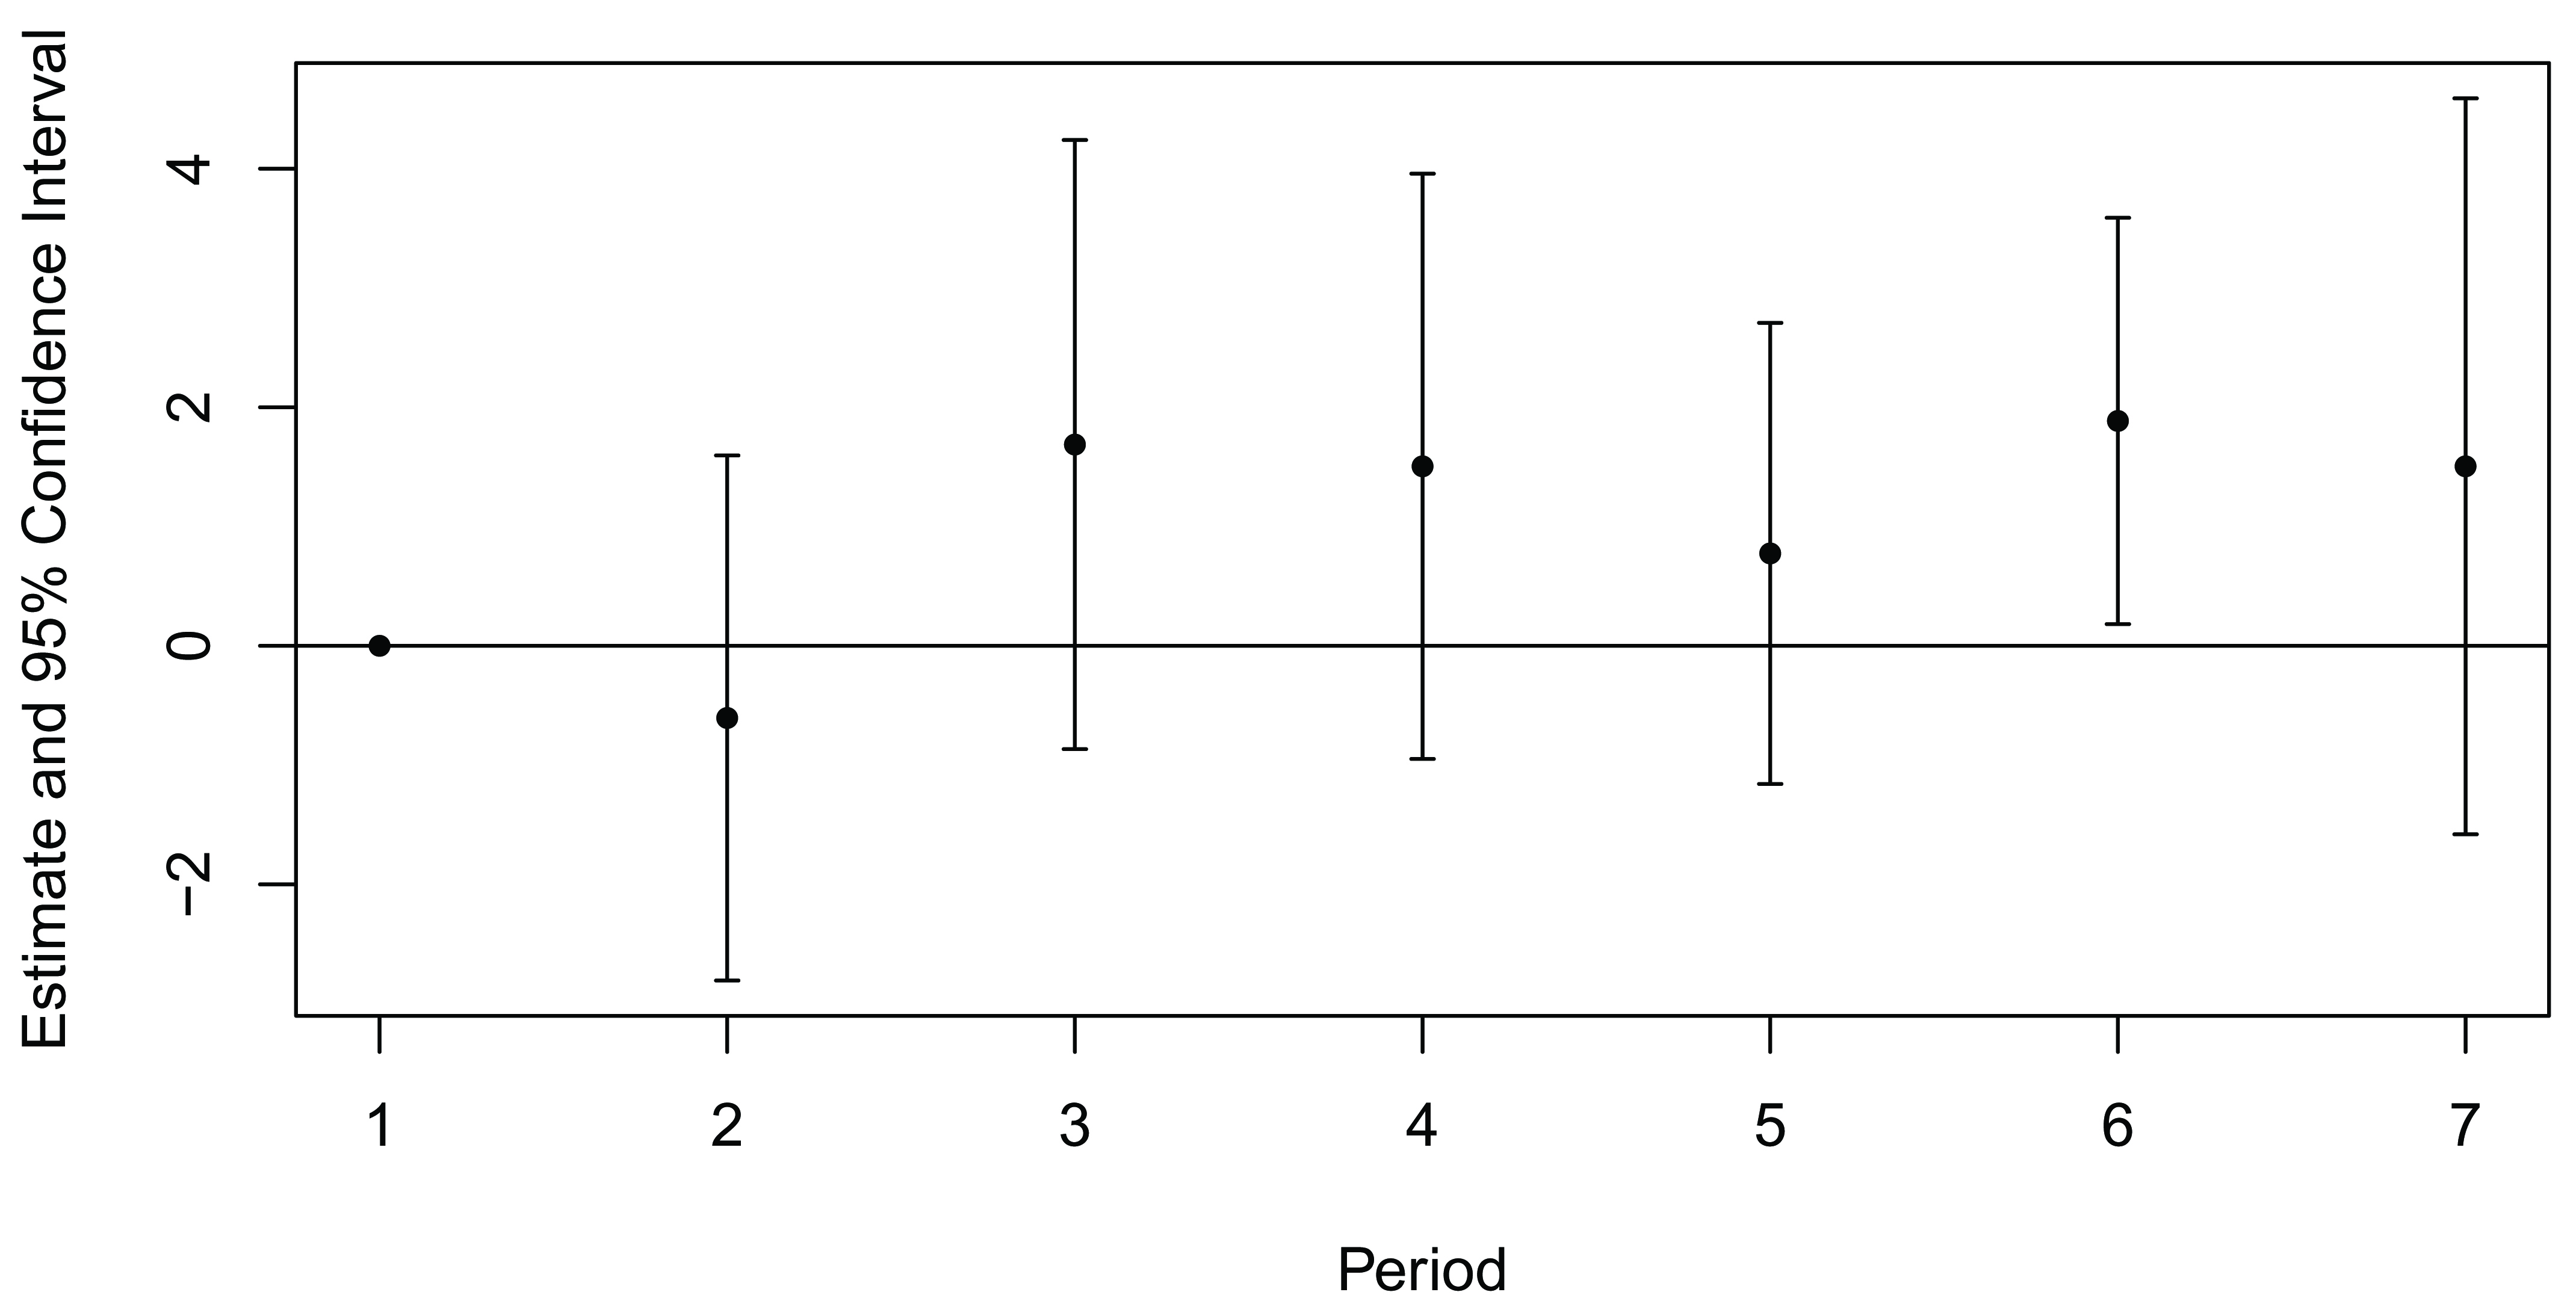
\includegraphics[scale=0.8]{Exhibits/food_insuf_event_study_with_controls.jpg}
\medskip 
\begin{minipage}{0.8\textwidth} 
{\footnotesize Notes: Sample ($N=1,729,108$) consists of respondents from Household Pulse Survey week 1 to week 40 who meet two criteria: 1) aged between 19 and 64 and 2) answered the question on Medicare coverage. The estimated model (shown in equation 1) include individual controls (state of residence, gender, pre-tax annual household income, race, Hispanic status, age, homeownership status,
marital status, educational attainment, number of dependents below 18, and household size). The dots represent the point estimates of the difference in food insufficiency between people with and without disabilities in each quarterly period (2 to 7) relative to period 1. Error bars represent 95 percent confidence intervals. Person-level weights are used in the analysis. \par}
\end{minipage}
\end{figure}

\begin{figure}[h!]\label{expens_dif_wc}
\caption{Difference in difficulty with expenses between people with and without disabilities over the quarterly periods relative to April-June 2020}
\centering
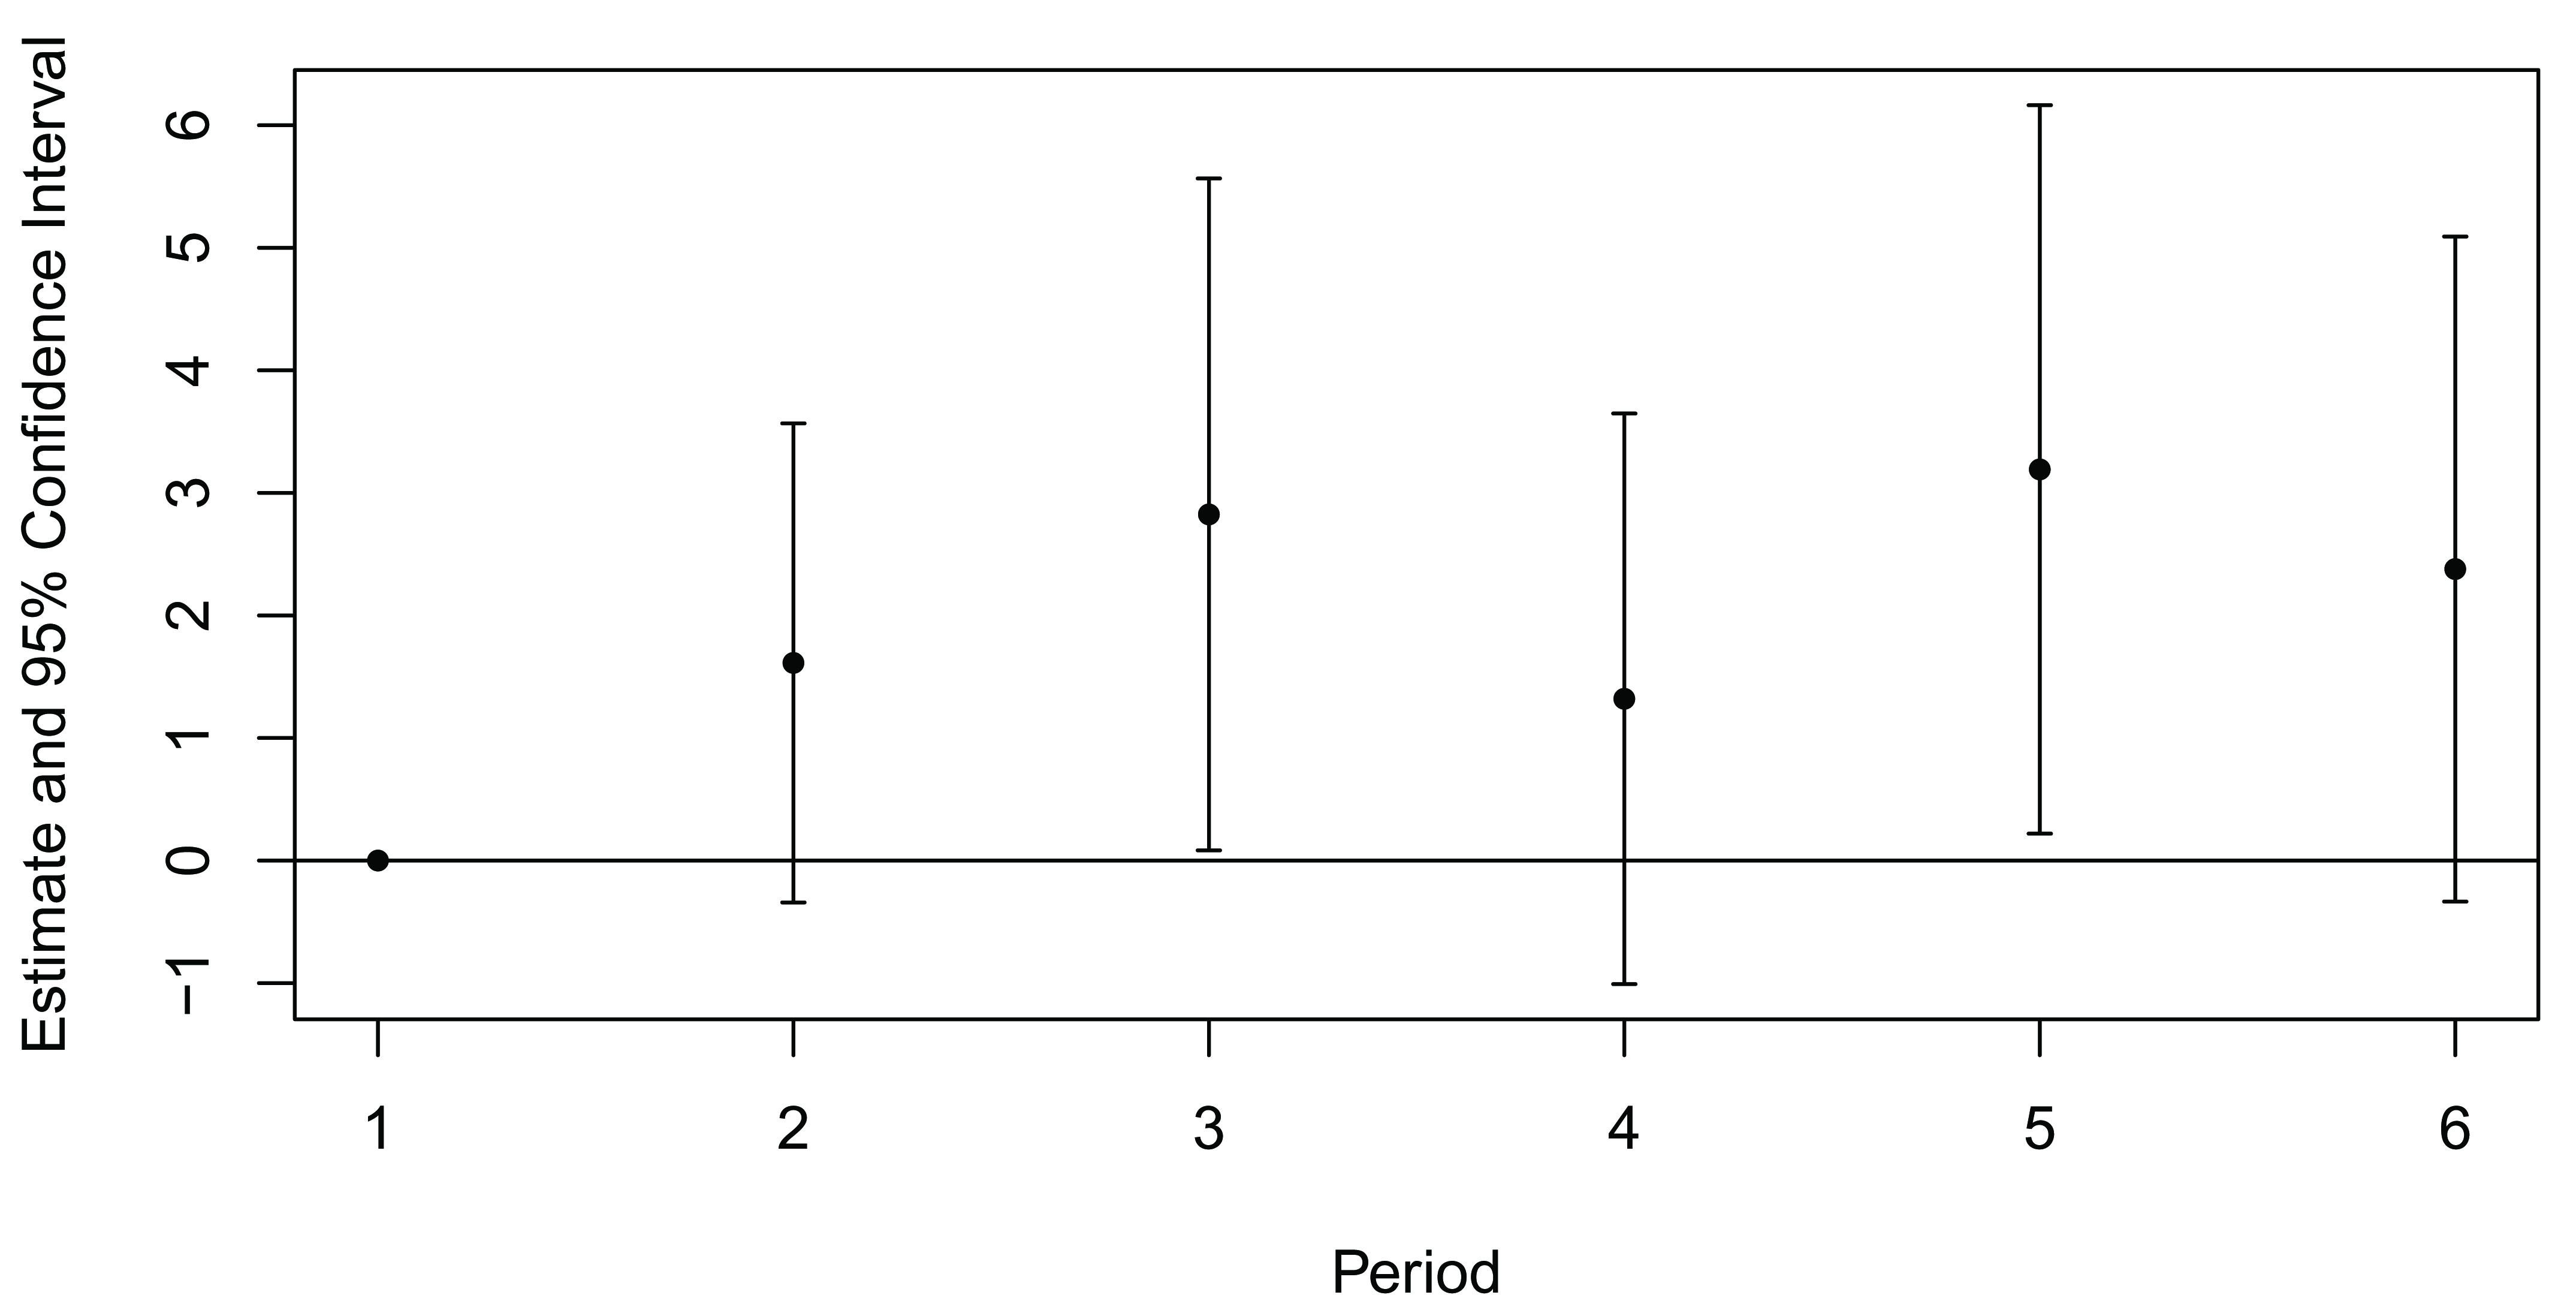
\includegraphics[scale=0.8]{Exhibits/expns_dif_event_study_with_controls.jpg}
\medskip 
\begin{minipage}{0.8\textwidth} 
{\footnotesize Notes: Sample ($N=1,104,824$) consists of respondents from Household Pulse Survey week 1 to week 40 who meet two criteria: 1) aged between 19 and 64 and 2) answered the question on Medicare coverage. The estimated model (shown in equation 1) include individual controls (state of residence, gender, pre-tax annual household income, race, Hispanic status, age, homeownership status,
marital status, educational attainment, number of dependents below 18, and household size). The dots represent the point estimates of the difference in difficulty with expenses between people with and without disabilities in each quarterly period (2 to 7) relative to period 1. Error bars represent 95 percent confidence intervals. Person-level weights are used in the analysis. \par}
\end{minipage}
\end{figure}


\begin{figure}[h!]\label{rent_conf_wc}
\caption{Difference in confidence in paying next month's rent/mortgage between people with and without disabilities over the quarterly periods relative to April-June 2020}
\centering
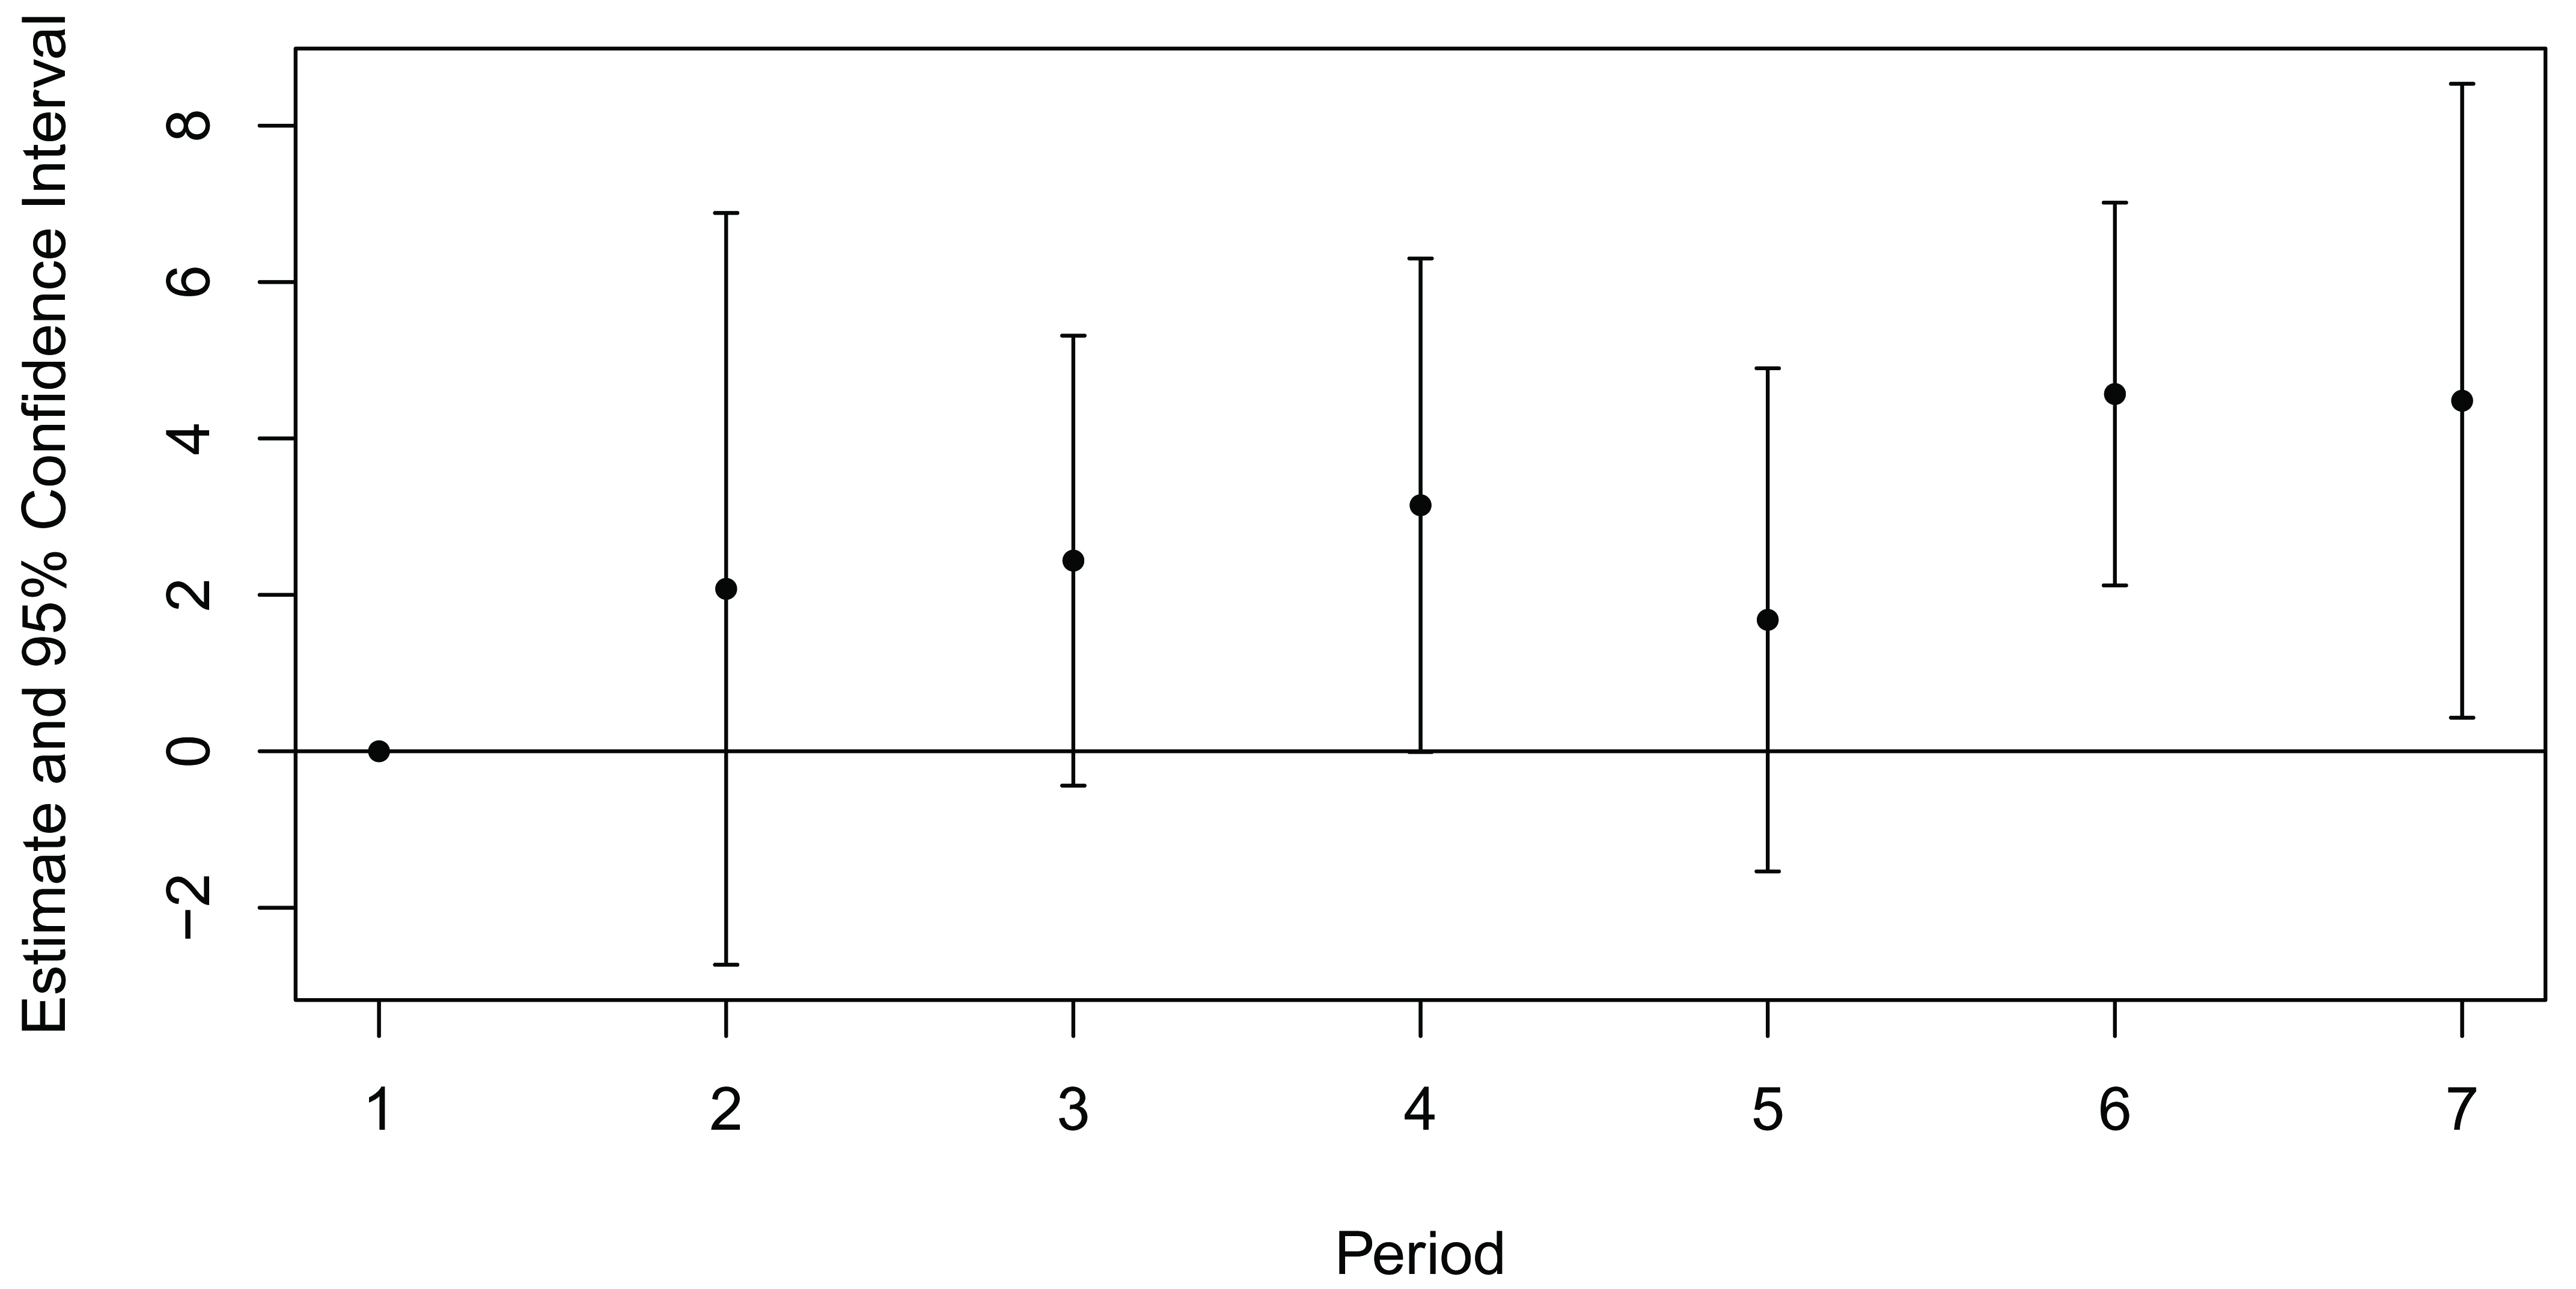
\includegraphics[scale=0.8]{Exhibits/mort_conf_event_study_with_controls.jpg}
\medskip 
\begin{minipage}{0.8\textwidth} 
{\footnotesize Notes: Sample ($N=1,395,349$) consists of respondents from Household Pulse Survey week 1 to week 40 who meet two criteria: 1) aged between 19 and 64 and 2) answered the question on Medicare coverage. The estimated model (shown in equation 1) include individual controls (state of residence, gender, pre-tax annual household income, race, Hispanic status, age, homeownership status,
marital status, educational attainment, number of dependents below 18, and household size). The dots represent the point estimates of the difference in confidence in paying next rent/mortgage payment between people with and without disabilities in each quarterly period (2 to 7) relative to period 1. Error bars represent 95 percent confidence intervals.Person-level weights are used in the analysis.  \par}
\end{minipage}
\end{figure}
 


 


 



 



 
\clearpage


\section*{References}
\renewcommand*{\refname}{\vspace*{-12mm}} 

%%  bib file with citations saved as "refs.bib"
\bibliography{refs}
\bibliographystyle{chicago}

\section*{Appendix}




\begin{table}[!h]
\caption{NFCS Summary Statistics}
\label{NFCS_Summstats}
 {
\def\sym#1{\ifmmode^{#1}\else\(^{#1}\)\fi}
\begin{tabular}{l*{5}{c}}
\hline\hline
                    &\multicolumn{2}{c|}{With Disabilities}&\multicolumn{2}{c|}{No Disabilities}&       Total\\ \hline
                    &2021&2018&2021&2018&  All     \\
\hline
Female              &        0.59&        0.58&        0.50&        0.50&        0.50\\
                    &      (0.49)&      (0.49)&      (0.50)&      (0.50)&      (0.50)\\
White               &        0.70&        0.66&        0.59&        0.59&        0.59\\
                    &      (0.46)&      (0.47)&      (0.49)&      (0.49)&      (0.49)\\
Black               &        0.13&        0.14&        0.13&        0.13&        0.13\\
                    &      (0.34)&      (0.34)&      (0.34)&      (0.34)&      (0.34)\\
Hispanic            &        0.11&        0.14&        0.18&        0.18&        0.18\\
                    &      (0.31)&      (0.35)&      (0.39)&      (0.39)&      (0.38)\\
Income $<$ \$25k       &        0.65&        0.64&        0.27&        0.22&        0.27\\
                    &      (0.48)&      (0.48)&      (0.44)&      (0.42)&      (0.44)\\
                    Income \$25k-\$75k    &        0.30&        0.31&        0.43&        0.44&        0.43\\
                    &      (0.46)&      (0.46)&      (0.49)&      (0.50)&      (0.49)\\
                    Income $>$ \$75k       &        0.05&        0.05&        0.30&        0.34&        0.30\\
                    &      (0.21)&      (0.22)&      (0.46)&      (0.47)&      (0.46)\\
Financial Well-being (0-100)&       41.45&       40.78&       50.26&       50.22&       49.63\\
                    &     (14.06)&     (14.09)&     (14.64)&     (14.61)&     (14.77)\\
Has Emergency Savings&        0.20&        0.18&        0.50&        0.46&        0.46\\
                    &      (0.40)&      (0.38)&      (0.50)&      (0.50)&      (0.50)\\
Financially Anxious&        0.68&        0.64&        0.61&        0.57&        0.59\\
                    &      (0.47)&      (0.48)&      (0.49)&      (0.50)&      (0.49)\\
Late CC Payment    &        0.22&        0.19&        0.21&        0.19&        0.20\\
                    &      (0.41)&      (0.39)&      (0.41)&      (0.39)&      (0.40)\\
Used AFS in Last 5 Years&        0.43&        0.40&        0.37&        0.33&        0.36\\
                    &      (0.49)&      (0.49)&      (0.48)&      (0.47)&      (0.48)\\
 Observations                   &        1481&        1402&       20136&       20177&       43196 \\
\hline\hline
\multicolumn{6}{l}{\footnotesize }\\
\end{tabular}
}

 \medskip 
\begin{minipage}{0.8\textwidth} 
{\footnotesize Notes: Means reported with standard deviations in parentheses. Data come from the 2018 and 2021 NFCS. We consider a respondent to have a disability if they answered ``Permanently sick, disabled, or unable to work" to the question ``Which of the following best describes your current employment or work status?" \par}
\end{minipage}
\end{table} 


%%%%%%%%%%%%%%%%%%%%%%%%%%%%%%%%%%%%%%%%%%%%%%%%%%%%%%%%
%SHED Summary Statistics%
%%%%%%%%%%%%%%%%%%%%%%%%%%%%%%%%%%%%%%%%%%%%%%%%%%%%%%%%
%\resizebox{\textwidth}{!}{%
\begin{table}[!ht]
    \centering
    \caption{SHED Summary Statistics}
    \begin{tabular}{llllll}
    \hline\hline
     &\multicolumn{2}{l|}{With Disabilities}&\multicolumn{2}{l|}{No Disabilities}&       Total\\ \hline
        ~ & 2018-2019 & 2020-2021 & 2018-2019 & 2020-2021 & All \\ \hline
        Female & 0.60  & 0.60  & 0.55  & 0.56  & 0.57  \\ 
        ~ & (0.49) & (0.49) & (0.50) & (0.50) & (0.50) \\ 
        White & 0.64  & 0.65  & 0.63  & 0.63  & 0.63  \\ 
        ~ & (0.48) & (0.48) & (0.48) & (0.48) & (0.48) \\ 
        Black & 0.14  & 0.13  & 0.10  & 0.10  & 0.11  \\ 
        ~ & (0.34) & (0.33) & (0.30) & (0.30) & (0.31) \\ 
        Hispanic & 0.14  & 0.15  & 0.16  & 0.18  & 0.16  \\ 
        ~ & (0.35) & (0.36) & (0.37) & (0.38) & (0.37) \\ 
        Income $<$ \$25k & 0.34  & 0.29  & 0.13  & 0.08  & 0.16  \\ 
        ~ & (0.47) & (0.45) & (0.34) & (0.27) & (0.37) \\ 
        Income \$25k-\$75k & 0.41  & 0.40  & 0.42  & 0.38  & 0.40  \\ 
        ~ & (0.49) & (0.49) & (0.49) & (0.48) & (0.49) \\ 
        Income $>$ \$75k & 0.25  & 0.31  & 0.45  & 0.54  & 0.44  \\ 
        ~ & (0.43) & (0.46) & (0.50) & (0.50) & (0.50) \\ 
        Spend$>$Income & 0.32  & 0.29  & 0.20  & 0.20  & 0.23  \\ 
        ~ & (0.46) & (0.46) & (0.40) & (0.40) & (0.42) \\ 
        Difficult to get by & 0.54  & 0.50  & 0.27  & 0.26  & 0.33  \\ 
        ~ & (0.50) & (0.50) & (0.44) & (0.44) & (0.47) \\ 
        No better off & 0.80  & 0.84  & 0.69  & 0.78  & 0.75  \\ 
        ~ & (0.40) & (0.36) & (0.46) & (0.41) & (0.43) \\ 
        Credit card balance & 0.73  & 0.73  & 0.58  & 0.50  & 0.59  \\ 
        ~ & (0.44) & (0.45) & (0.49) & (0.50) & (0.49) \\ 
        Observations & 1489 & 1162 & 4719 & 3613 & 10983 \\ \hline\hline
    \end{tabular}
    \label{SHED_Sumstats}
     \medskip 
\begin{minipage}{0.85\textwidth} 
{\footnotesize Notes: Means reported with standard deviations in parentheses. Data come from the 2018- 2021 SHED. We consider a respondent to have a disability if they answered ``Yes" to the question ``Did Health/medical limitations or disability  contribute to you not working/not working as much as you wanted last month?" \par}
\end{minipage}
\end{table}

%%%%%%%%%%%%%%%%%%%%%%%%%%%%%%%%%%%%%%%%%%%%%%%%%%%%%%%%
% HPS summary statistics (food_insuf) %
%%%%%%%%%%%%%%%%%%%%%%%%%%%%%%%%%%%%%%%%%%%%%%%%%%%%%%%%
\begin{table}[!ht]
    \centering
    \caption{Summary Statistics of the Food Insufficiency Analytical Sample from the HPS}
    \begin{tabular}{llll}
    \hline \hline
        ~ & With Disabilities & No Disabilities & Total \\ \hline
        Female & 0.67  & 0.61  & 0.62  \\ 
        ~ & (0.47) & (0.49) & (0.49) \\ 
        White & 0.75  & 0.81  & 0.80  \\ 
        ~ & (0.43) & (0.39) & (0.40) \\ 
        Black & 0.12  & 0.08  & 0.08  \\ 
        ~ & (0.33) & (0.27) & (0.28) \\ 
        Hispanic & 0.11  & 0.10  & 0.10  \\ 
        ~ & (0.31) & (0.30) & (0.30) \\ 
        Income $<$ \$25k & 0.32  & 0.09  & 0.10  \\ 
        ~ & (0.46) & (0.28) & (0.30) \\ 
        Income \$25k-\$75k & 0.38  & 0.32  & 0.33  \\ 
        ~ & (0.49) & (0.47) & (0.47) \\ 
        Income $>$ \$75k & 0.23  & 0.53  & 0.51  \\ 
        ~ & (0.42) & (0.50) & (0.50) \\ 
        Food Insufficient & 0.17  & 0.07  & 0.08  \\ 
        ~ & (0.38) & (0.26) & (0.27) \\ 
        Observations & 94079 & 1635029 & 1729108 \\ 
        \hline \hline
    \end{tabular}
    \label{hps_food_sample}
    \medskip 
\begin{minipage}{0.7\textwidth} 
{\footnotesize Notes: Means reported with standard deviations in parentheses. Data come from the HPS. We consider a respondent to have a disability if they were aged 19-64 and enrolled in Medicare. \par}
\end{minipage}
\end{table}

%%%%%%%%%%%%%%%%%%%%%%%%%%%%%%%%%%%%%%%%%%%%%%%%%%%%%%%%
% HPS summary statistics (diff_expns) %
%%%%%%%%%%%%%%%%%%%%%%%%%%%%%%%%%%%%%%%%%%%%%%%%%%%%%%

\begin{table}[!ht]
    \centering
    \caption{Summary Statistics of the Difficulty with Expenses Analytical Sample from the HPS}
    \begin{tabular}{llll}
    \hline \hline
        ~ & With Disabilities & No Disabilities & Total \\ \hline
        Female & 0.67  & 0.61  & 0.62  \\ 
        ~ & (0.47) & (0.49) & (0.49) \\ 
        White & 0.76  & 0.81  & 0.81  \\ 
        ~ & (0.43) & (0.39) & (0.40) \\ 
        Black & 0.12  & 0.08  & 0.08  \\ 
        ~ & (0.33) & (0.27) & (0.27) \\ 
        Hispanic & 0.11  & 0.10  & 0.10  \\ 
        ~ & (0.31) & (0.31) & (0.31) \\ 
        Income $<$ \$25k & 0.31  & 0.08  & 0.10  \\ 
        ~ & (0.46) & (0.28) & (0.29) \\ 
        Income \$25k-\$75k & 0.37  & 0.31  & 0.31  \\ 
        ~ & (0.48) & (0.46) & (0.46) \\ 
        Income $>$ \$75k & 0.23  & 0.53  & 0.51  \\ 
        ~ & (0.42) & (0.50) & (0.50) \\ 
        Difficulty with expenses & 0.45  & 0.26  & 0.27  \\ 
        ~ & (0.50) & (0.44) & (0.44) \\ 
        Observations & 59367 & 1045457 & 1104824 \\ 
        \hline \hline
    \end{tabular}
    \label{hps_diff_expns_sample}
    \medskip 
\begin{minipage}{0.8\textwidth} 
{\footnotesize Notes: Means reported with standard deviations in parentheses. Data come from the HPS. We consider a respondent to have a disability if they were aged 19-64 and enrolled in Medicare. \par}
\end{minipage}
\end{table}


%%%%%%%%%%%%%%%%%%%%%%%%%%%%%%%%%%%%%%%%%%%%%%%%%%%%%%%%
% HPS summary statistics (rent_conf) %
%%%%%%%%%%%%%%%%%%%%%%%%%%%%%%%%%%%%%%%%%%%%%%%%%%%%%%%%
\begin{table}[!ht]
    \centering
    \caption{Summary Statistics of the Confidence in Paying Rent/Mortgage Payments Analytical Sample from the HPS}
    \begin{tabular}{llll}
    \hline \hline
        ~ & With Disabilities & No Disabilities & Total \\ \hline
        Female & 0.68  & 0.62  & 0.62  \\ 
        ~ & (0.47) & (0.49) & (0.49) \\ 
        White & 0.74  & 0.81  & 0.80  \\ 
        ~ & (0.44) & (0.39) & (0.40) \\ 
        Black & 0.14  & 0.09  & 0.09  \\ 
        ~ & (0.34) & (0.28) & (0.28) \\ 
        Hispanic & 0.11  & 0.11  & 0.11  \\ 
        ~ & (0.32) & (0.31) & (0.31) \\ 
        Income $<$ \$25k & 0.34  & 0.09  & 0.10  \\ 
        ~ & (0.47) & (0.28) & (0.30) \\ 
        Income \$25k-\$75k & 0.39  & 0.33  & 0.34  \\ 
        ~ & (0.49) & (0.47) & (0.47) \\ 
        Income $>$ \$75k & 0.23  & 0.54  & 0.53  \\ 
        ~ & (0.42) & (0.50) & (0.50) \\ 
        Not confident in paying rent/mortgage & 0.22  & 0.14  & 0.14  \\ 
        ~ & (0.42) & (0.35) & (0.35) \\ 
        Observations & 67009 & 1328340 & 1395349 \\ 
        \hline \hline
    \end{tabular}
    \label{hps_diff_expns_sample}
        \medskip 
\begin{minipage}{0.9\textwidth} 
{\footnotesize Notes: Means reported with standard deviations in parentheses. Data come from the HPS. We consider a respondent to have a disability if they were aged 19-64 and enrolled in Medicare. \par}
\end{minipage}
\end{table}

\clearpage
 

\includepdf[scale=1]{back.pdf}
 
\end{document}